\lab{Python}{NumPy and SciPy}{NumPy and SciPy}
%\label{lab:NumPySciPy}

\section*{Why Arrays?}
Let's begin with a simple demonstration of why arrays are important for numerical computation.
Why use arrays when Python already has a reasonably efficient list object?
In this demonstration, we will try squaring a matrix.
The matrix will be represented as a two dimensional list (i.e. a list of lists).

The following is a function that will accept two matrices (two dimensional list), $A$ and $B$, and return $AB$ following the usual rules of matrix multiplication.
\lstinputlisting[style=fromfile]{arr_mult.py}
We can initialize a $k \times k$ ``array" of integers like this:
\begin{lstlisting}
>>> k = 10
>>> A = [range(i, i+k) for i in range(0, k**2, k)]
\end{lstlisting}

\begin{problem}
Time how long this function takes to square matrices for increasing values of \li{k}.
In IPython you can time how long it takes for a line of code to execute by prefacing it with \li{\%timeit}, as in \li{\%timeit range(100)}.

Now import NumPy and create a NumPy array, \li{A}, and square it.
\li{A*A} does \emph{not} square the array, but rather multiplies \li{A} with itself element by element.
To get matrix multiplication for NumPy arrays, you must use \li{np.dot} or the \li{dot()} method of an array like this:
\begin{lstlisting}
import numpy as np
A = np.array([range(i, i+k) for i in range(0, k**2, k)])
np.dot(A, A)
\end{lstlisting}
Time how long NumPy takes to square arrays for increasing sizes of \li{k}.
What do you notice about the time needed to square a two dimensional list vs. a two dimensional NumPy array?
\end{problem}

% Below is a comparison of runtimes needed to square a matrix
% \begin{center}
% \begin{tabular}{|c|l|l|}
% \hline
%  Data Structure & Size & Time (s) \\ \hline
%  Python List & $1\times1$ & 0.0000181198 \\ \cline{2-3}
%       & $10\times10$ & 0.0002758503 \\ \cline{2-3}
%       & $100\times100$ & 0.1336028576 \\ \cline{2-3}
%       & $1000\times1000$ & 200.4009799957 \\ \hline \hline
%  NumPy Array & $1\times1$ & 0.0000298023 \\ \cline{2-3}
%       & $10\times10$ & 0.0000109673 \\ \cline{2-3}
%       & $100\times100$ & 0.0009210110 \\ \cline{2-3}
%       & $1000\times1000$ & 2.1682999134 \\ \hline
% \end{tabular}
%
% \end{center}

The reason for the drastic speed difference is that Python, as a high level interpreted language, tends to be slower than lower level compiled languages.
The algorithms implemented in NumPy are heavily optimized and are usually implemented in C or Fortran.
Instead of operating purely in Python, they use Python to run code that is written and optimized in other languages.
NumPy interfaces with some of the best known packages for doing computational linear algebra and can be used to write relatively fast programs.

Lists are still faster for anything that involves a varying lengths of data.
If you are appending to your data or deleting items, consider using lists instead of arrays since both of these operations require the creation of a new array.

\section*{NumPy}
NumPy is a fundamental package for scientific computing with Python.
It provides an efficient $n$-dimensional (arbitrary dimensional) array object for fast computations.
These arrays are commonly known as \emph{ndarrays}.
This lab will focus on how to use these powerful objects.
NumPy is commonly imported as shown below.
NumPy also provides a matrix object which is designed to behave like matrices in MATLAB.
It is strongly encouraged to use NumPy arrays instead of NumPy matrices, despite their convenience.
Numpy is typically imported with \li{import numpy as np}.
First, it will be useful to explain certain concepts and terms used to describe NumPy arrays.

\subsection*{Arbitrary Dimensions}
One, two, and three dimensional arrays are easy to visualize.
But how do we visualize a four, ten, or fifteen dimensional array?
NumPy arrays are best thought of as arrays within arrays.
A one dimensional array consists of only elements.
A two dimensional array is really just an array containing arrays which contain elements.
Extending this metaphor, a three dimensional array is an array of arrays of arrays.
Let's define a random three dimensional array.
\begin{lstlisting}
>>> arr = np.random.randint(50, size=(5, 4, 3))
\end{lstlisting}
% Arrays are objects in Python.
% For those who are familiar with object oriented programming, it is worth noting that many of the functions we discuss here are also implemented as methods of \li{ndarray} objects.
Two simple attributes of arrays that describe the number of elements in an array are \li{shape} and \li{size}
\li{shape} gives information about the size of the array in each dimension.
\li{Size} gives the total number of elements in every dimension of the array.
\begin{lstlisting}
>>> arr.shape
(5, 4, 3)
>>> arr.size
60
\end{lstlisting}
Indexing always starts at $0$.
Also, like Python lists, negative indices are valid and count backwards from the end of the array.
We will discuss indexing in more detail later in this lab.
\begin{lstlisting}
>>> arr[0, 0, 0] #returns the first element of arr
>>> arr[-1, -1, -1] #returns the last element of arr
\end{lstlisting}

\section*{Creating Arrays}
NumPy has several functions for creating and initializing arrays.
When creating an array, we can, optionally, specify the data type that is stored in the 
array.
NumPy arrays are homogeneous, meaning that all elements in an array must have the same 
datatype.
Let's look at a few of the ways we can create arrays in NumPy.
\begin{itemize}
\item \li{np.array}: Makes an array from a Python list or tuple.
Can also be used to make a new array based on an old one, possibly with a changed datatype.
\item \li{np.empty}: Allocates an array of a specific size without initializing the elements.
\item \li{np.empty_like}: Allocates a new uninitialized array with the same shape and type as the input array.
\item \li{np.ones}: Allocates and array and initializes each element to $1$.
\item \li{np.ones_like}: Allocates a new array of ones with the same shape and type as the input array.
\item \li{np.zeros}: Allocates an array and initializes each element to $0$.
\item \li{np.zeros_like}: Allocates a new array of zeros with the same shape and type as the input array.
\item \li{np.identity}: Allocates a 2D array with ones along the main diagonal and zeros everywhere else.
\item \li{np.random.rand}: Allocates an array of random floating point values between 0 and 1.
\end{itemize}

\subsection*{Universal Functions (ufuncs)}
NumPy and SciPy include a wide variety of functions that are designed to operate on 
arrays.
Such functions, which take in an array and return an array of the same size and
datatype, are called \emph{universal functions}. To illustrate this point, consider 
the universal function \li{numpy.sin} and the standard function \li{math.sin}. If $A$ 
is an array of floats (of any size), \li{math.sin(A)} throws an error, whereas 
\li{numpy.sin(A)} returns an array of floats containing the sines of the entries of $A$. 
Other simple examples from NumPy include \li{cos}, \li{sqrt}, \li{exp}, and 
\li{log} all the way to special functions like \li{polygamma} in the \li{scipy.misc} submodule.
There are far more functions available in NumPy than could possibly be included here, so you will want to become familiar with the NumPy and SciPy documentation at \url{docs.scipy.org/doc/}.
If you need to do any sort of simple operation on an array, there is very often a function there to do it.
These functions are almost always faster and more convenient than iterating through the whole array.

Most of these functions also allow you to specify an array for the output.
It is useful in cases where you would like to avoid unnecessary memory allocation.
The output array does need to be the correct shape to store the output.
For example:
\begin{lstlisting}
>>> np.exp(A, out=A) #take exp(A) and store result in A
\end{lstlisting}

Other useful examples are \li{max}, \li{min}, \li{absolute}, and \li{average}.
Each of these operations also allows you to specify whether you want to operate across a particular axis or over the whole array.
For example:
\begin{lstlisting}
>>> np.max(A, axis=0) #max along axis 0
\end{lstlisting}
The above example returns a row of A which represents the maximum of all the rows of A.
If we had set \li{axis=1}, it would have taken the maximum of all the columns.
If, for purposes of broadcasting (discussed later) you need the output of one of these functions to have the same number of dimensions as the original array, you can also include the argument \li{keepdims=True}.

\subsection*{Indexing Arrays}
\subsubsection*{Array Views and Copies}
Before we begin accessing arrays, it is important to understand that NumPy has two 
ways of slicing an array.
Slice operations always return a \emph{view} and fancy indexing always returns a \emph{copy}.
Understand that even though they may look the same, views and copies are very different.

Views are special arrays that reference other arrays.
Changing elements in a view changes the array it references.
Below, we demonstrate the behavior of a view.
Notice that \li{c} looks like a copy of \li{b} even though it is not.
\begin{lstlisting}
>>> b = np.reshape(np.arange(25), (5,5))
>>> b
array([[ 0,  1,  2,  3,  4],
       [ 5,  6,  7,  8,  9],
       [10, 11, 12, 13, 14],
       [15, 16, 17, 18, 19],
       [20, 21, 22, 23, 24]])
>>> c = b[:] #looks like c is a copy of b
>>> c
array([[ 0,  1,  2,  3,  4],
       [ 5,  6,  7,  8,  9],
       [10, 11, 12, 13, 14],
       [15, 16, 17, 18, 19],
       [20, 21, 22, 23, 24]])
>>> id(c) == id(b) #We have unique objects
False
>>> c[2] = 500
>>> c
array([[  0,   1,   2,   3,   4],
       [  5,   6,   7,   8,   9],
       [500, 500, 500, 500, 500],
       [ 15,  16,  17,  18,  19],
       [ 20,  21,  22,  23,  24]])
>>> b #changing c also changed b!
array([[  0,   1,   2,   3,   4],
       [  5,   6,   7,   8,   9],
       [500, 500, 500, 500, 500],
       [ 15,  16,  17,  18,  19],
       [ 20,  21,  22,  23,  24]])
\end{lstlisting}
The reason that changing the array \li{c} also changed the array \li{b} is because \li{c} 
and \li{b} contain references to the same data in memory, even though they are different 
Python objects.
Views reduce the overhead of making copies of arrays and are useful when we want to change 
certain parts of the array.

A copy of an array is a separate array that is allocated separately.
An array can be copied using the \li{copy()} function.
\begin{lstlisting}
>>> b = np.reshape(np.arange(25), (5, 5))
>>> b
array([[ 0,  1,  2,  3,  4],
       [ 5,  6,  7,  8,  9],
       [10, 11, 12, 13, 14],
       [15, 16, 17, 18, 19],
       [20, 21, 22, 23, 24]])
>>> c = np.copy(b)
>>> c is b #we still have separate objects
False
>>> c[2] = 500
>>> c
array([[  0,   1,   2,   3,   4],
       [  5,   6,   7,   8,   9],
       [500, 500, 500, 500, 500],
       [ 15,  16,  17,  18,  19],
       [ 20,  21,  22,  23,  24]])
>>> b
array([[ 0,  1,  2,  3,  4],
       [ 5,  6,  7,  8,  9],
       [10, 11, 12, 13, 14],
       [15, 16, 17, 18, 19],
       [20, 21, 22, 23, 24]])
\end{lstlisting}
Changing the data in a copy of an array does not affect the data in the original array.
The two arrays address different locations in memory.

\subsubsection*{Slices}
Each element of an array has a unique address that we can use to retrieve that element.
Indexing and slicing of NumPy arrays follows syntax that is similar to the syntax used 
with Python lists.
We will demonstrate on a simple 2D array.
Remember that slicing arrays always return a view of an array.
\begin{lstlisting}
>>> arr = np.reshape(np.arange(25), (5,5))
>>> arr
array([[ 0,  1,  2,  3,  4],
       [ 5,  6,  7,  8,  9],
       [10, 11, 12, 13, 14],
       [15, 16, 17, 18, 19],
       [20, 21, 22, 23, 24]])
>>> arr[0, 0] #access the first element
0
>>> arr[-1, -1] #access the last element
24
>>> arr[0] #access the first row
array([0, 1, 2, 3, 4])
\end{lstlisting}
We can access ranges of elements using Python lists.
We can also more concisely select ranges using the \li{arr[start:stop:step]} range notation.
\begin{lstlisting}
>>> arr[::2] #get every other row, equivalent to arr[range(0, len(arr), 2)]
array([[ 0,  1,  2,  3,  4],
       [10, 11, 12, 13, 14],
       [20, 21, 22, 23, 24]])
>>> arr[::2, ::2] #get every other row and every other column
array([[ 0,  2,  4],
       [10, 12, 14],
       [20, 22, 24]])
>>> arr[3:, 3:] #extract lower right 2x2 subarray
array([[18, 19],
       [23, 24]])
>>> arr[:, 1] #extract second column
array([ 1,  6, 11, 16, 21])
\end{lstlisting}
Operations like those above are called array slicing.
Array slices are views of portions of the data of the original array.
They do not copy any data. It is vital to keep this in mind when making changes 
to the data in array slices.

\subsubsection*{Fancy Indexing}
It is possible to index an array with an object such as a list or an array, 
but in this case NumPy behaves a little differently.
This feature is commonly referred to as fancy indexing.
One difference is that fancy indices always return a copy of an array instead of a view.
There are two types of fancy indexing: boolean and integer.
Boolean indexing returns an array of \li{True} or \li{False} values depending on some 
evaluating condition.
\begin{lstlisting}
>>> bmask = (arr > 15) & (arr < 23)
>>> bmask
array([[False, False, False, False, False],
       [False, False, False, False, False],
       [False, False, False, False, False],
       [False,  True,  True,  True,  True],
       [ True,  True,  True,  False,  False]], dtype=bool)
>>> arr[bmask]
array([16, 17, 18, 19, 20, 21, 22])
>>> arr[(arr > 15) & (arr < 23)] #this is the shortened form
array([16, 17, 18, 19, 20, 21, 22])
>>> arr[~bmask] #invert the mask
array([ 0,  1,  2,  3,  4,  5,  6,  7,  8,  9, 10, 11, 12, 13, 14, 15, 23, 24])
\end{lstlisting}
\begin{lstlisting}
>>> arr[(0, 2, 4), (0, 2, 4)] #grab every other element of diagonal
array([ 0, 12, 24])
>>> arr[range(0, 5, 2), range(0, 5, 2)] #same as above, but with ranges
array([ 0, 12, 24])
>>> arr[:, [0, -1]] #grab first and last column
array([[ 0,  4],
       [ 5,  9],
       [10, 14],
       [15, 19],
       [20, 24]])
\end{lstlisting}

Though fancy indexing does not return a view of the array, it \emph{can} be used for assignment.
For example, we will set all values of an array that are less than .5 to 0 as follows:
\begin{lstlisting}
>>> from numpy.random import rand
>>> A = rand(10, 10)
>>> A[A<.5] = 0.
\end{lstlisting}

\begin{problem}
Generate a random $1000 \times 1000$ array \li{A}.
Now create an uninitialized array \li{B} with all the same attributes as \li{A}.
Now do the following 100 times:
\begin{itemize}
\item Overwrite \li{B} so that it is an array of new random values like \li{A}.
This can be done like this: \li{B[:] = rand(1000,1000)}
\item Use fancy indexing to make \li{A} the maximum of \li{A} and \li{B}.
\end{itemize}
Now take \li{exp(A)} and have NumPy store the output directly in \li{A}.
Take the maximum along the vertical axis and average the result.
The final number should be very close to $e$.
\end{problem}

\section*{The Transpose and Other Useful Operations}
You may have noticed that we already used the \li{reshape()} function.
It allows us to make a new view of our array with a desired shape.
The new shape must make an array of the same size as the original array.
If we need to take the transpose of an array \li{A}, we can use the transpose attribute 
of the array, \li{A.T}, which will give us a new view of the same array with the order 
of the dimensions reversed.
The NumPy \li{transpose()} function will also do this.
Remember that both of these methods will return views of the original array and not new 
arrays.

The functions \li{flatten}, \li{vstack}, \li{hstack}, and \li{copy} are examples of 
functions that will return new arrays.
Given a $3 \times 3$ array, \li{flatten} will return a new copy of the array with 
shape \li{(9,)}. The functions \li{vstack} and \li{hstack} will return new copies of the 
input array with possibly different shapes. See the documentation for the details. The 
function \li{copy} simply returns an exact copy of the array. 

The syntax \li{A[:]} will return a new view of \li{A} that is identical to \li{A}.
This doesn't sound all that useful, but if you want to override the values in an array, 
this syntax can be extremely handy.
For example:
\begin{lstlisting}
>>> import numpy as np
>>> from numpy.random import rand
>>> A = rand(100)
>>> B = rand(100)
>>> A[:] = 0 #sets each entry in A to 0
>>> A[:] = B #copies the data from B into A
\end{lstlisting}

\begin{problem}
Operations that create completely new arrays are often slower than operations that create views because allocating an array can be time consuming.
Create a $1000 \times 1000$ array \li{A} of floating point values.
Compare the speed of the operations \li{A.reshape(A.size)} and \li{A.flatten()} (here we are calling the methods of the arrays, these are the same as \li{np.reshape(A, A.size)}, and \li{np.flatten(A)} respectively).
Why is there such a difference in speed?
What is the difference between their output?
What about \li{A.reshape((1,A.size))}?
The reason \li{A.flatten()} takes longer is that it is allocating a new array in memory and copying all of the values from the input array into this new array.  In contrast, \li{A.reshape()} simply changes they way the array is read from memory by changing the shape of the array.  It doesn't touch any of the data of the array.  There are times, though, when creating a copy is desired behavior.
\end{problem}

\begin{problem}
One good application of array slicing is the Jacobi method for solving Laplace's 
equation, which is used to model steady-state heat flow, on a square.
This is an example of a simple iterative method.
In this case we will modify our array in place.
Make a function that accepts an array and a tolerance as input and does the following:
\begin{enumerate}
\item Copy the array into a new array
\item Create a variable to track the difference between the arrays.
Initialize it as the tolerance.
\item While the difference is greater than or equal to the tolerance
\begin{enumerate}
	\item set all points that are not on an edge of the new array equal to the average of 
    their 4 immediate neighbors.
    Use the values from the old array for this computation.
    This should only take one line and should be based entirely on array slicing.
    (Hint: given a 2D array \li{A}, the slice \li{A[1:-1,1:-1]} references all non-edge 
    entries, \li{A[:-2,1:-1]} references the left neighbors, and \li{A[1:-1,2:]} 
    references the bottom neighbors.)
	\item update the difference to be the maximum of the absolute value of the new array minus the old one.
	\item copy the values from the new array into the old one (without creating a new array).
\end{enumerate}
\end{enumerate}

Now use the following code to generate a plot of your results
\begin{lstlisting}
>>> from matplotlib import pyplot as plt
>>> from mpl_toolkits.mplot3d import Axes3D
>>> n = 100
>>> tol = .0001
>>> U = np.ones((n, n))
>>> U[:,0] = 100                        # set north boundary condition
>>> U[:,-1] = 100                       # set south boundary condition
>>> U[0] = 0                            # set west boundary condition
>>> U[-1] = 0                           # set east boundary condition
>>> laplace(U, tol)                     # U has been changed in place
>>> X = np.linspace(0, 1, n)
>>> Y = np.linspace(0, 1, n)
>>> X, Y = np.meshgrid(X, Y)
>>> fig = plt.figure()
>>> ax = fig.gca(projection='3d')
>>> ax.plot_surface(X, Y, U, rstride=5)
>>> plt.show()
\end{lstlisting}

\begin{figure}[H]
\centering
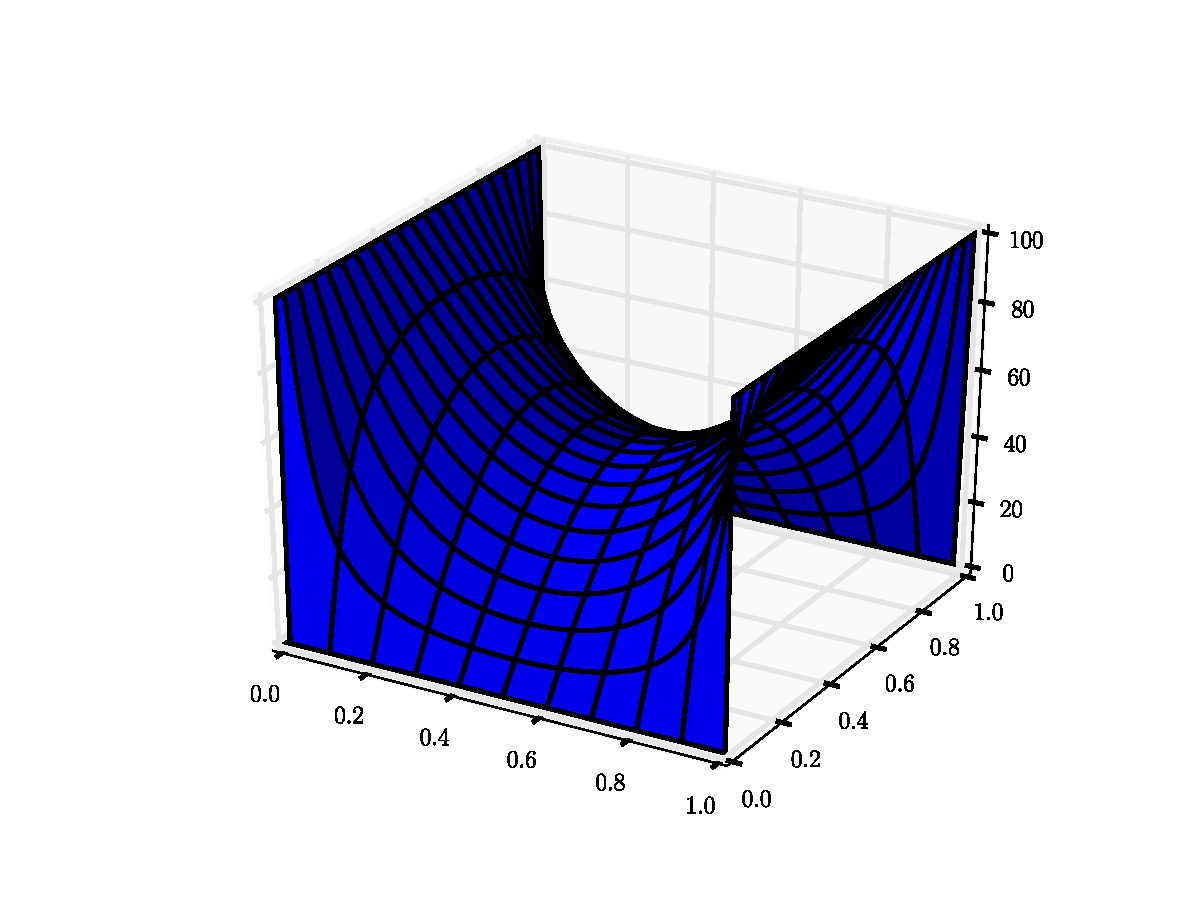
\includegraphics[width=.75\textwidth]{laplace.pdf}
\end{figure}
\end{problem}

\section*{Array Broadcasting}
Array broadcasting allows NumPy to work effectively with arrays of sizes that don't match 
exactly. This can be useful in a host of different situations, and often saves both the 
amount of typing that is necessary and the amount of memory required for computations. 
There are four basic rules to determine the behavior of broadcasted arrays.
\begin{enumerate}
\item All input arrays of lesser dimension than the input array with largest dimension 
    have 1's prepended to their shapes.
\item The size in each dimension of the output shape is the maximum of all the input sizes 
    in that dimension.
\item An input can be used in the calculation if its size in a particular dimension either 
    matches the output size in that dimension, or has a size exactly 1.
\item If an input has a dimension size of 1 in its shape, the first data entry in that 
    dimension will be used for all calculations along that dimension.
\end{enumerate}

One simple example is multiplying a two dimensional array by a set of numbers along its rows or columns.
Run the following lines of code and consider their output:
\begin{lstlisting}
>>> import numpy as np
>>> A = np.ones((3, 3))
>>> B = np.vstack(np.array([1, 2, 3,]))
>>> A * B #multiplies the rows of A by each entry of B
array([[ 1.,  1.,  1.],
       [ 2.,  2.,  2.],
       [ 3.,  3.,  3.]])
>>> A * B.T #multiplies the columns of A by each entry of B
array([[ 1.,  2.,  3.],
       [ 1.,  2.,  3.],
       [ 1.,  2.,  3.]])
\end{lstlisting}

For a more detailed description of array broadcasting rules, see \url{http://docs.scipy.org/doc/numpy/user/basics.broadcasting.html}.

When working with multi-dimensional arrays, it can be useful to create new views of your arrays that change the order of the dimensions.
This will give you greater control over how different arrays are broadcast together.
This can be done by taking a transpose, using the \li{rollaxis} function, or using the \li{swapaxes} function.
The \li{rollaxis} function will take a given axis and change the ordering of the axes of the array so that that particular axis appears at a new place.
The order of the other axes will not be changed.
The \li{swapaxes} function will swap the placement of two axes.
Note that all three of these options create views of the previous array.
There is no copying of data involved.

\begin{problem}
Create a $100\times100\times3$ array of integers taking values in the range [0, 256] 
(using the function \li{numpy.random.randint} with appropriate arguments). 
Such an array can represent a RGB image of $100\times100$ pixels, where each pixel 
is associated with an array of three integers indicating the amounts of red, green, and 
blue color present in that pixel, respectively. Using array broadcasting, multiply the 
red and green values by $.5$. Such an operation will tone down the red and green colors 
and make the image appear bluer. 
\end{problem}

\section*{Arrays and Memory}
When working with large arrays, we need to be aware of memory and performance issues that 
arise from how the arrays are stored in memory.
If we want to know how much memory an array uses to store its elements, we can use 
\li{arr.nbytes}.
The number of bytes is dependent on the data type or \emph{dtype} of the array.
The data types that NumPy uses are different from Python data types.
An integer in NumPy is not the same as an integer Python.
Remembering this is vital.
NumPy uses low level data types to speed up calculations.
However, these data types are susceptible to a problem called \emph{overflow}.
A 64 bit integer has enough bits to represent integers between $-2^{63}$ (that's 
$-9,223,372,036,854,775,808$) and $2^{63} - 1$.
If we have an array with $-2^{63}$ and we decide to subtract 1, the integer wraps around 
and becomes $2^{63} - 1$!  If we wish to reduce memory usage, we can use smaller integer 
types.
NumPy has support for 8, 16, 32, and 64 bit integers.
\begin{lstlisting}
>>> arr.dtype
dtype('int64')
>>> arr.nbytes
480
>>> arr.astype('int32').nbytes
240
\end{lstlisting}

Arrays can be stored in various \emph{orders} in memory, which dictate how 
the array is laid out in memory.
Two common layouts are C order and Fortran order.
C ordered arrays are also known as row-major arrays.
This means that the fastest changing index corresponds to the rows of the array.
This is because rows are stored in contiguous blocks in memory.
Fortran ordered arrays are column-major.
Another common way of saying this is that an array is C contiguous or Fortran contiguous.
Not all arrays are C contiguous or Fortran contiguous, but it is useful to understand the 
distinction. These issues become important when you need to optimize your code to run as 
fast as possible. 
% we need more discussion here, with some examples as well. Why is it important to know?

\section*{Saving Arrays}
It is often useful to save an array as a file.
NumPy provides several easy methods for saving and loading array data.
\begin{table*}[h]
\begin{tabular}{|l|l|}
\hline
\li{np.save(file, arr)} & Save an array to a binary file \\
\li{np.savez(file, *arrs)} & Save multiple arrays to a binary file \\
\li{np.savetxt(file, arr)} & Save an array to a text file \\
\hline
\end{tabular}
\end{table*}

\begin{table*}[h]
\begin{tabular}{|l|l|}
\hline
\li{np.load(file)} & Load and return an array from a binary file \\
\li{np.loadtxt(file)} & Load and return an array from text file \\
\hline
\end{tabular}
\end{table*}

Let's practice saving an array to a file and loading it again.
Note that, when saving an array, NumPy automatically appends the extension \li{.npy} if it is not already present.
\begin{lstlisting}
a = np.arange(30)
np.save('test_arr', a)
new_a = np.load('test_arr.npy')
np.savez('test_multi', a=a, new_a=new_a)
arrs = np.load('test_multi.npz')
\end{lstlisting}
The variable \li{arrs} points to a dictionary object with the keys \li{a} and \li{new_a} which reference the arrays that have been saved.
The \li{.npz} file extension is the file type used to store multiple arrays.

\section*{SciPy}
SciPy is a Python library that provides many easy-to-use, efficient algorithms for all types of scientific computing.
It is designed to work with NumPy arrays.
It is therefore important to master the use of NumPy arrays.
Many of the algorithms needed to solve problems in these lab manuals are implemented in SciPy.
SciPy is organized into packages grouped by problem type.
There are packages for statistics, optimization, signal processing, linear algebra, etc.
You can find a SciPy tutorial as well as a reference list to its various packages at 
\url{http://docs.scipy.org/doc/scipy/reference/}. 
% \begin{table}[h]
% \centering
% \begin{tabular}{|l|l|}
% \hline
% cluster & Clustering package \\
% constants & Physical and mathematical constants and units \\
% fftpack & Fast Fourier transforms \\
% integrate & Integration package \\
% interpolate & Interpolation package \\
% io & Data input/output from various formats \\
% linalg & Linear algebra functions \\
% misc & Various utilities that can't be classified elsewhere \\
% ndimage & Multi-dimensional image processing \\
% odr & Orthogonal distance regression \\
% optimize & Optimization and root finding \\
% signal & Signal processing package \\
% sparse & Two dimensional sparse matrices \\
% sparse.linalg & Sparse matrix linear algebra functions \\
% sparse.csgraph & Fast graph algorithms based on sparse matrices \\
% spatial & Spatial algorithms and data structures \\
% special & Special functions \\
% stats & Statistical functions \\
% mstats & Statistical functions for masked arrays \\
% \hline
% \end{tabular}
% \caption{SciPy subpackages}
% \end{table}

One of the primary packages that we will be using is \li{scipy.linalg}.
Even though NumPy also has \li{numpy.linalg}, using \li{scipy.linalg} is preferred.
% Reasons for this include the fact that \li{scipy.linalg} is more fully featured and is 
% always compiled with BLAS/LAPACK support (this support is optional in NumPy).
% NumPy's linear algebra library should only be used to avoid adding scipy as a dependency.
Let's look at a few of the routines in SciPy's linear algebra module.
\begin{lstlisting}
>>> import numpy as np
>>> from scipy import linalg as la
>>> arr = np.array([[2, 3], [5, 7]])
>>> la.det(arr) #find the determinant of arr
-1.0000000000000018
>>> la.inv(arr) #find the inverse of arr
array([[-7.,  3.],
       [ 5., -2.]])
>>> la.eig(arr) #return eigenvalues and corresponding eigenvectors
(array([-0.10977223+0.j,  9.10977223+0.j]),
 array([[-0.81797819, -0.38876264],
       [ 0.57524923, -0.92133794]]))
\end{lstlisting}

There are also many extension packages for more specialized problems such as machine learning and natural language processing.
These packages are called \emph{SciKits}.
These kits augment the functionality of SciPy.
They are designed to work efficiently with NumPy arrays.
Some portions of these packages may someday be included in SciPy itself, but many of these packages are still incomplete or in development.
However, they can still be useful. You can find a list of these extension packages as well 
as links to the documentation at \url{http://scikits.appspot.com/scikits}.

% \begin{table}[h]
% \centering
% \begin{tabular}{|l|l|}
% \hline
% scikit-aero & Aeronautical engineering routines \\
% scikit-commpy & Digital communications in Python \\
% scikit-fmm & Fast marching method implementation \\
% scikit-image & Image processing functions \\
% scikit-learn & Machine learning and data mining routines \\
% scikit-rf & RF/Microwave engineering routines \\
% ann & Approximate nearest neighbor search using KDTrees \\
% audiolab & Make noise from NumPy arrays \\
% bootstrap & Bootstrap confidence interval estimation \\
% bvp1lg & Multi-point boundary value problem solver \\
% bvp\_solver & Two-point boundary value problem solver \\
% cuda & Python interface to CUDA libraries \\
% datasmooth & Data smoothing routines \\
% eartho & Earth observation functions \\
% fitting & Data fitting framework \\
% hydroclimpy & Environmental time series for Python \\
% odes & Ordinary differential equation solver for Python \\
% samplerate & High quality audio resampling \\
% scattpy & Light scattering methods for Python \\
% sparse & Sparse matrix package \\
% statsmodels & Statistical computations and models \\
% talkbox & Set of routines for speech/signal processing \\
% timeseries & Time series manipulation \\
% vectorplot & Vector fields plotting algorithms \\
% \hline
% \end{tabular}
% \caption{SciKits extend the functionality of SciPy.}
% \end{table}
